\paragraph{QuizziPedia::Front-End::Controllers::TopicKeywordsController}
\begin{figure} [ht]
	\centering
	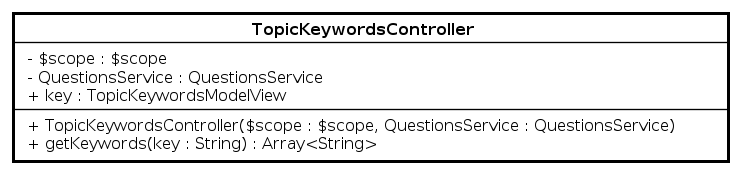
\includegraphics[scale=0.45]{UML/Classi/Front-End/QuizziPedia_Front-end_Controller_TopicKeywordsController.png}
	\caption{QuizziPedia::Front-End::Controllers::TopicKeywordsController}
\end{figure} \FloatBarrier
\begin{itemize}
	\item \textbf{Descrizione}: questa classe permette di gestire il recupero delle parole chiave di un questionario;
	\item \textbf{Utilizzo}: fornisce le funzionalità per il recupero delle parole chiave durante la creazione di un questionario;
	\item \textbf{Relazione con altre classi}:
	\begin{itemize}
		\item \textit{IN} \texttt{TopicKeywordsModelView}: ; 
		\item \textit{IN} \texttt{QuestionsService}: questa classe permette di ottenere domande esistenti e salvare nuove domande;
	\end{itemize}
	\item \textbf{Attributi}:
	\begin{itemize}
		\item \texttt{-} \texttt{\$scope: \$scope} \\
		Campo dati contenente un riferimento all’oggetto \$scope creato da \textit{Angular\ped{G}}, viene utilizzato come mezzo di comunicazione tra il controller e la view. Contiene gli oggetti che definiscono il model dell’applicazione;
		\item \texttt{-} \texttt{QuestionService: QuestionService}\\ 
		Permette, tra le altre cose, di ottenere le parole chiave a partire da una stringa passata.
		\item \texttt{+} \texttt{key: TopicKeywordsModelView} \\
		Oggetto di tipo \texttt{CreateQuestionnaireView}. All'interno di esso sono presenti le variabili e i metodi necessari per il \textit{Two-Way Data-Binding\ped{G}} tra la direttiva \texttt{TopicKeywordsDirective} e il controller \texttt{TopicKeywordsController};
	\end{itemize}
	\item \textbf{Metodi}:
	\begin{itemize}
		\item \texttt{+} \texttt{TopicKeywordsController(\$scope: \$scope)} \\Metodo costruttore della classe. \\
		\textbf{Parametri}:
		\begin{itemize}
			\item \texttt{-} \texttt{\$scope: \$scope} \\
			Campo dati contenente un riferimento all’oggetto \$scope creato da \textit{Angular\ped{G}}. Viene utilizzato come mezzo di comunicazione tra il controller e la view. Contiene gli oggetti che definiscono il viewmodel e il model dell’applicazione; 
		\end{itemize}
		\item \texttt{-} \texttt{getKeywords(key: String): String[]}: \\ Metodo che ritorna le parole che hanno a che fare con key
	\end{itemize}
	\textbf{Parametri}:
	\begin{itemize}
		\item \texttt{key: String}: parametro che identifica la stringa con la quale cercare le keywords. 
	\end{itemize}
\end{itemize}